\chapter{Evaluatie}
\label{chap:evaluatie}

In dit hoofdstuk wordt de vergelijking uitgevoerd op basis van de vijf actieve vergelijkingscriteria uit hoofdstuk \ref{chap:vergelijkingscriteria}, namelijk populariteit~(\ref{sec:evaluatie-populariteit}), productiviteit~(\ref{sec:evaluatie-productiviteit}), gebruik~(\ref{sec:evaluatie-gebruik}), ondersteuning~(\ref{sec:evaluatie-ondersteuning}) en performantie~(\ref{sec:evaluatie-performantie}). 
Daarna zullen deze vijf vergelijkingscriteria in sectie~\ref{sec:evaluatie-spinnenweb} worden samengevat.

%%%%%%%%%%%%%%%%%%%%%%%%%%%%%%%%%%%%%%%%%%%%%%%%%%%%%%%%%%%%%%%%%%%%%%%%

\section{Populariteit} % 2 blz inclusief google trends
\label{sec:evaluatie-populariteit}

De populariteit van de vier raamwerken op 8 mei 2013 wordt weergegeven in tabel~\ref{tabel:evaluatie-populariteit}. 
%TODO ref naar formule (tim), Tim: ok?
Voor de score van populariteit wordt naar formule \ref{eq:populariteit} verwezen die de som neemt van Twitter volgers, \gh{} sterren, \gh{} \term{forkers}, \so{} vragen en \fb{} vind-ik-leuks.

%TODO ik zie dat de twitter tweets in de totaalscore worden opgenomen, terwijl er in het vergelijkingshoofdstuk niets daarover staat in de formule?
\begin{table}
\centering
\pgfplotstabletypeset[
  begin table=\begin{tabular}{p{8cm} p{1cm} p{1cm} p{1cm} p{1cm}},
  end table=\end{tabular},
  skip coltypes=true,
  col sep=comma,
  string type,
  header=true,
  columns={Populariteit,ST,Kendo,jQM,Lungo},
  columns/Populariteit/.style={column name=\textbf{Populariteit}, column type={l}},  
  columns/jQM/.style={column name=\textbf{\jqma}, column type={c}},
  columns/ST/.style={column name=\textbf{\sta}, column type={c}},
  columns/Lungo/.style={column name=\textbf{\lungoa}, column type={c}},
  columns/Kendo/.style={column name=\textbf{\kendoa}, column type={c}},
  every head row/.style={
    before row=\toprule,
    after row=\midrule},
  every last row/.style={
  	before row=\midrule,
    after row=\bottomrule}
]{tabellen/populariteit.csv}
\caption{Overzicht van populariteit op 8 mei 2013.}
\label{tabel:evaluatie-populariteit}
\end{table}

\kendo{} neemt de eerste plaats voor zich dankzij het zeer groot aantal vind-ik-leuks op \fb.
\jqm{} en \st{} slepen respectievelijk een tweede en derde plaats in de wacht, ondanks het feit dat ze in de literatuur de meest aangehaalde raamwerken zijn~\cite{David2011,Firtman2013,Hales2012,Oeflman2011}. 
Als laatste eindigt \lungo{} met een opmerkelijke lage populariteit op \so{} en \fb.
Bij het kijken naar de totaalscore kunnen twee groepen worden waargenomen, enerzijds de groep bestaande uit \kendo{} en \jqm{} en anderzijds de groep bestaande uit \st{} en \lungo{}.

Op Twitter heeft \jqm{} de meeste volgers, gevolgd door \kendo.
Op de voorlaatste plaats komt \lungo{}, maar als het aantal \term{tweets} wordt uitgezet ten opzichte van het aantal volgers, kan er gesteld worden dat \lungo{} het meest actief is.
\jqm{} en \kendo{} hebben een vergelijkbare activiteit bij het sturen van \term{tweets}.
\st{} heeft het minst aantal volgers en het aantal verstuurde \term{tweets} is slechts 1.
Deze \term{tweet} verwijst naar de Twitter-account van Sencha zelf.
Sencha heeft een kleine 3.000 \term{tweets} en een kleine 20.000 volgers.

In tegenstelling tot \jqm{} en \lungo{} bevinden \kendo{} en \st{} zich niet op \gh{}.
Zelfs indien \gh{} wordt weggelaten, blijft de rangschikking ongewijzigd.
De opvatting van Capgemini dat enkel \term{open-soruce} raamwerken populair zijn, wordt ontkracht door deze cijfers.

\kendo{} verwijst op zijn website voor ondersteuning rechtstreeks naar de fora op \so{}. 
Toch blijft de populariteit van \kendo{} op \so{} lager dan die van \jqm{}.
\st{} behaalt de voorlaatste plaats, maar opvallend is \lungo{} die slechts een dertigtal vragen op \so{} heeft en dus op de laatste plaats eindigt.

\kendo{} en \jqm{} hebben beide een fanpgina op \fb{} opgericht in respectievelijk november 2011 en augustus 2010.
De fanpgina van \kendo{} heeft dus in een kortere tijd veel meer vind-ik-leuks opgeleverd dat de eerder opgerichte fanpgina van \jqm{}.
De verschillende producten van \kendo{} worden geaggregeerd op één fanpagina. 
\st{} en \lungo{} hebben enkel een interessepagina op \fb.
Dit verklaart het grote verschil in vind-ik-leuks op \fb.
Het aantal vind-ik-leuks bepaald de populariteit in grote mate.
Indien deze vind-ik-leuks worden weggelaten, wisselen \jqm{} en \kendo{} van plaats.
De auteurs zijn van mening dat \fb{} een belangrijk sociaal netwerk is.
Daarenboven kost het ook geen geld om een fanpagina aan te maken.
Hierdoor kan \fb{} niet uit het populariteitscriterium worden weggelaten.  

Deze populariteit werd ook iedere week bijgehouden over een periode van een $7$ weken.
Opvallend is de sterke opmars van \kendo{} in deze korte periode.
Dit komt grotendeels door het enorm stijgend aantal vind-ik-leuks op \fb{}.
De andere drie raamwerken stijgen gestaag.

%\begin{figure}
%  \centering
%  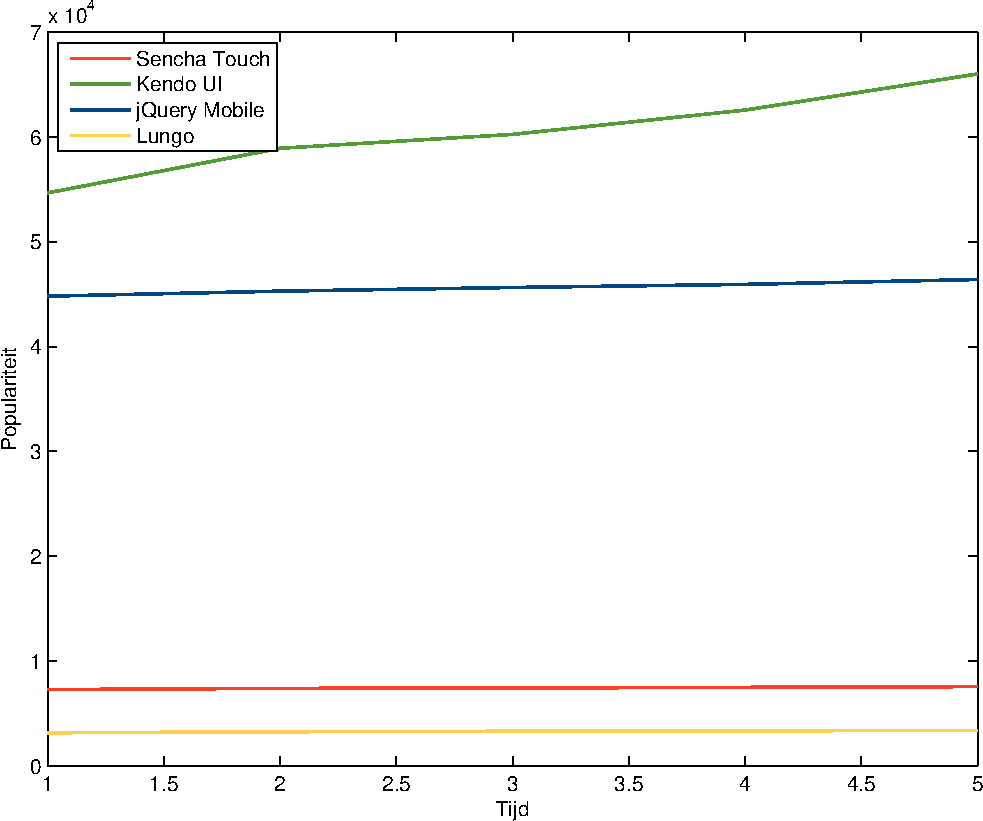
\includegraphics[width=0.8\textwidth]{figuren/populariteit-tijd.pdf}
%  \caption{Populariteit waargenomen over de periode van 15 april tot 22 mei 2013.}
%  \label{fig:populariteit-evolutie}
%\end{figure}

Als laatste wordt de populariteit aan de hand van Google Trends bekeken op figuur~\ref{fig:google-trends}.
Duidelijk is dat hier \jqm{} de grote winnaar is.
Sinds 2011 maakt het raamwerk een grote opmars door het uitbrengen van de eerste stabiele versie~1.0.
Tussen versie~1.2 (uitgekomen in oktober 2012) en versie~1.3 (uitgekomen in februari 2013) daalt de interesse met $40\%$.
Dit valt te verklaren doordat de nieuwe interesse in versie~1.2 daalt, maar weer opwakkerd bij de aankondiging van versie~1.3. 
Een gelijkaardige trend kan ook bij \st{} opgemerkt worden.
\st{} kende een piek in maart 2012 bij het uitbrengen van \st{}~2.0.
Sinds begin 2012 maakt \kendo{} een opmars en als de trend zich verder zet, zal het \st{} inhalen.
Dit komt overeen met de waargenomen opmars van \kendo{} tijdens de periode van $7$ weken.
\lungo{} is nauwelijks op de grafiek waarneembaar.

\begin{figure}
  \centering
  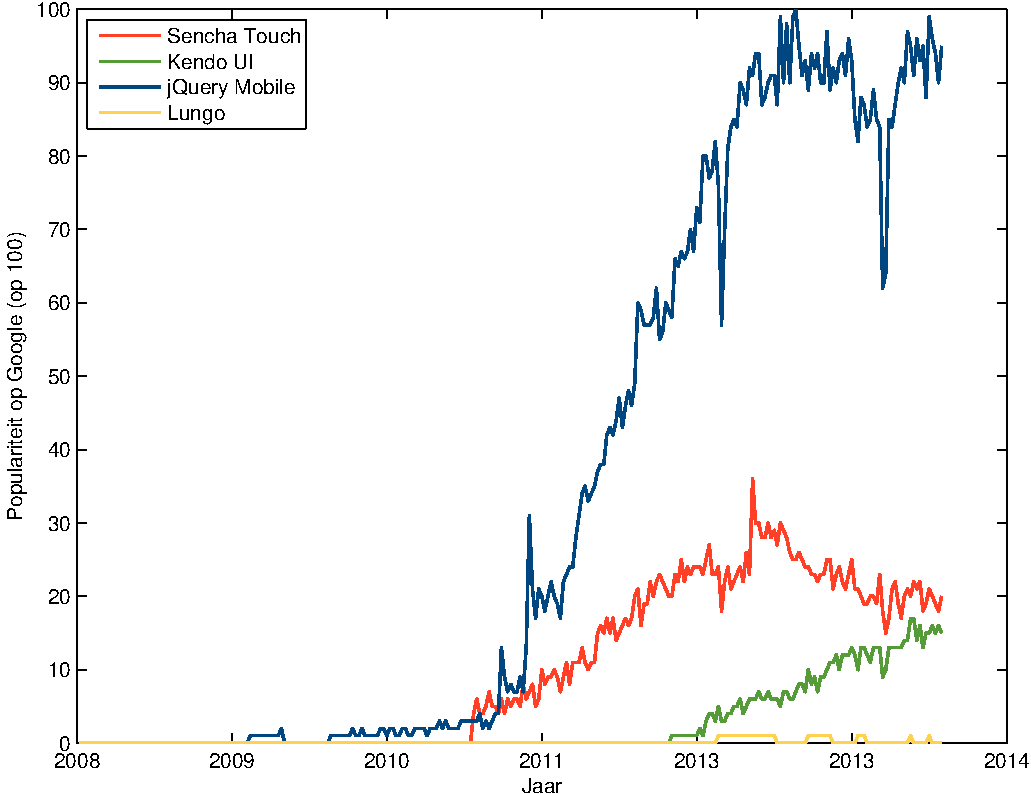
\includegraphics[width=0.8\textwidth]{figuren/google-trends.pdf}
  \caption{Populariteit op Google Trends waargenomen van januari 2008 tot heden waarbij een resultaat van 100 overeenkomt met de grootste zoekinteresse~\cite{Google2012a}.}
  \label{fig:google-trends}
\end{figure}